\documentclass{beamer}
\usepackage{float}
\usepackage{enumerate}
\usepackage{graphicx}
\usepackage {tikz}
\usepackage{caption}
\usepackage{subcaption}
\usepackage{booktabs}
\usepackage{csquotes}
\usepackage{upquote}
\usepackage{xcolor}
\usepackage[most]{tcolorbox}
\usetheme{Madrid}

\usepackage[english]{babel}
\usepackage[utf8x]{inputenc}
\usepackage{amsmath}
\usepackage{graphicx}
\usepackage[colorinlistoftodos]{todonotes}


\title{Weakly supervised semantic segmentation}
\author{You}

\begin{document}
	
	\title{Weakly Supervised Semantic Segmentation}
	
	% A subtitle is optional and this may be deleted
	%\subtitle{Optional Subtitle}
	
	\author{Goutam YG, Haris Iqbal, Marimuthu Kalimuthu}
	% - Give the names in the same order as the appear in the paper.
	% - Use the \inst{?} command only if the authors have different
	%   affiliation.
	
	\institute[Saarland University] % (optional, but mostly needed)
	{
		Department of Computer Science\\
		Saarland University
	}
	
	\subject{Theoretical Computer Science}
	
	\begin{frame}
		\titlepage
	\end{frame}
	
	% Section and subsections will appear in the presentation overview
	% and table of contents.
	\section{First Main Section}
	
	\subsection{First Subsection}
	
	\begin{frame}{Problem Statement}
		\begin{itemize}
			\item {
				Segmenting an image using scribbles as partial labellings
			}
			\item {
				Challenging because of: ill-defined boundaries, articulations, noise etc.,
			}
		\end{itemize}
	\end{frame}
	
	
	
	\begin{frame}{Motivation}
		\begin{itemize}
			\item {
				Obtaining dense segmentation results manually is both costly and time-consuming.
			}
			\item{
				Unsupervised approaches do not yield good results in general
			}
			
			\item{With scribble annotations, it is possible to achieve high accurate results  }
			
	\begin{figure}[H]
		\begin{center}
			\includegraphics[width=0.50\textwidth]{scribble.jpg}
			\caption{Scribble Annotated}
		\end{center}			
	\end{figure}

		\end{itemize}
	\end{frame}
	
	
	
	\begin{frame}{Related Works}
		\begin{block}{}
			\begin{itemize}
				\item Dilation Network (Yu et al., 2016)
				\item ScribbleSup (Lin et al., 2016)
				\item SegNet (Kendall et al., 2015)
				\item FCNs (Long et al., 2015)		
			\end{itemize}
		\end{block}
		
	\end{frame}
	
	
	
	\begin{frame}{Our Proposed Strategy}
		%may not be relevant # TODO: more details
	\begin{figure}[H]
		\begin{center}
			\includegraphics[width=0.95\textwidth]{architecture.png}
			\caption{Architecture of our System}
		\end{center}			
	\end{figure}
		
	\end{frame}
		
	
	
	\begin{frame}{Visualization}
		\begin{figure}[H]
			\begin{center}
				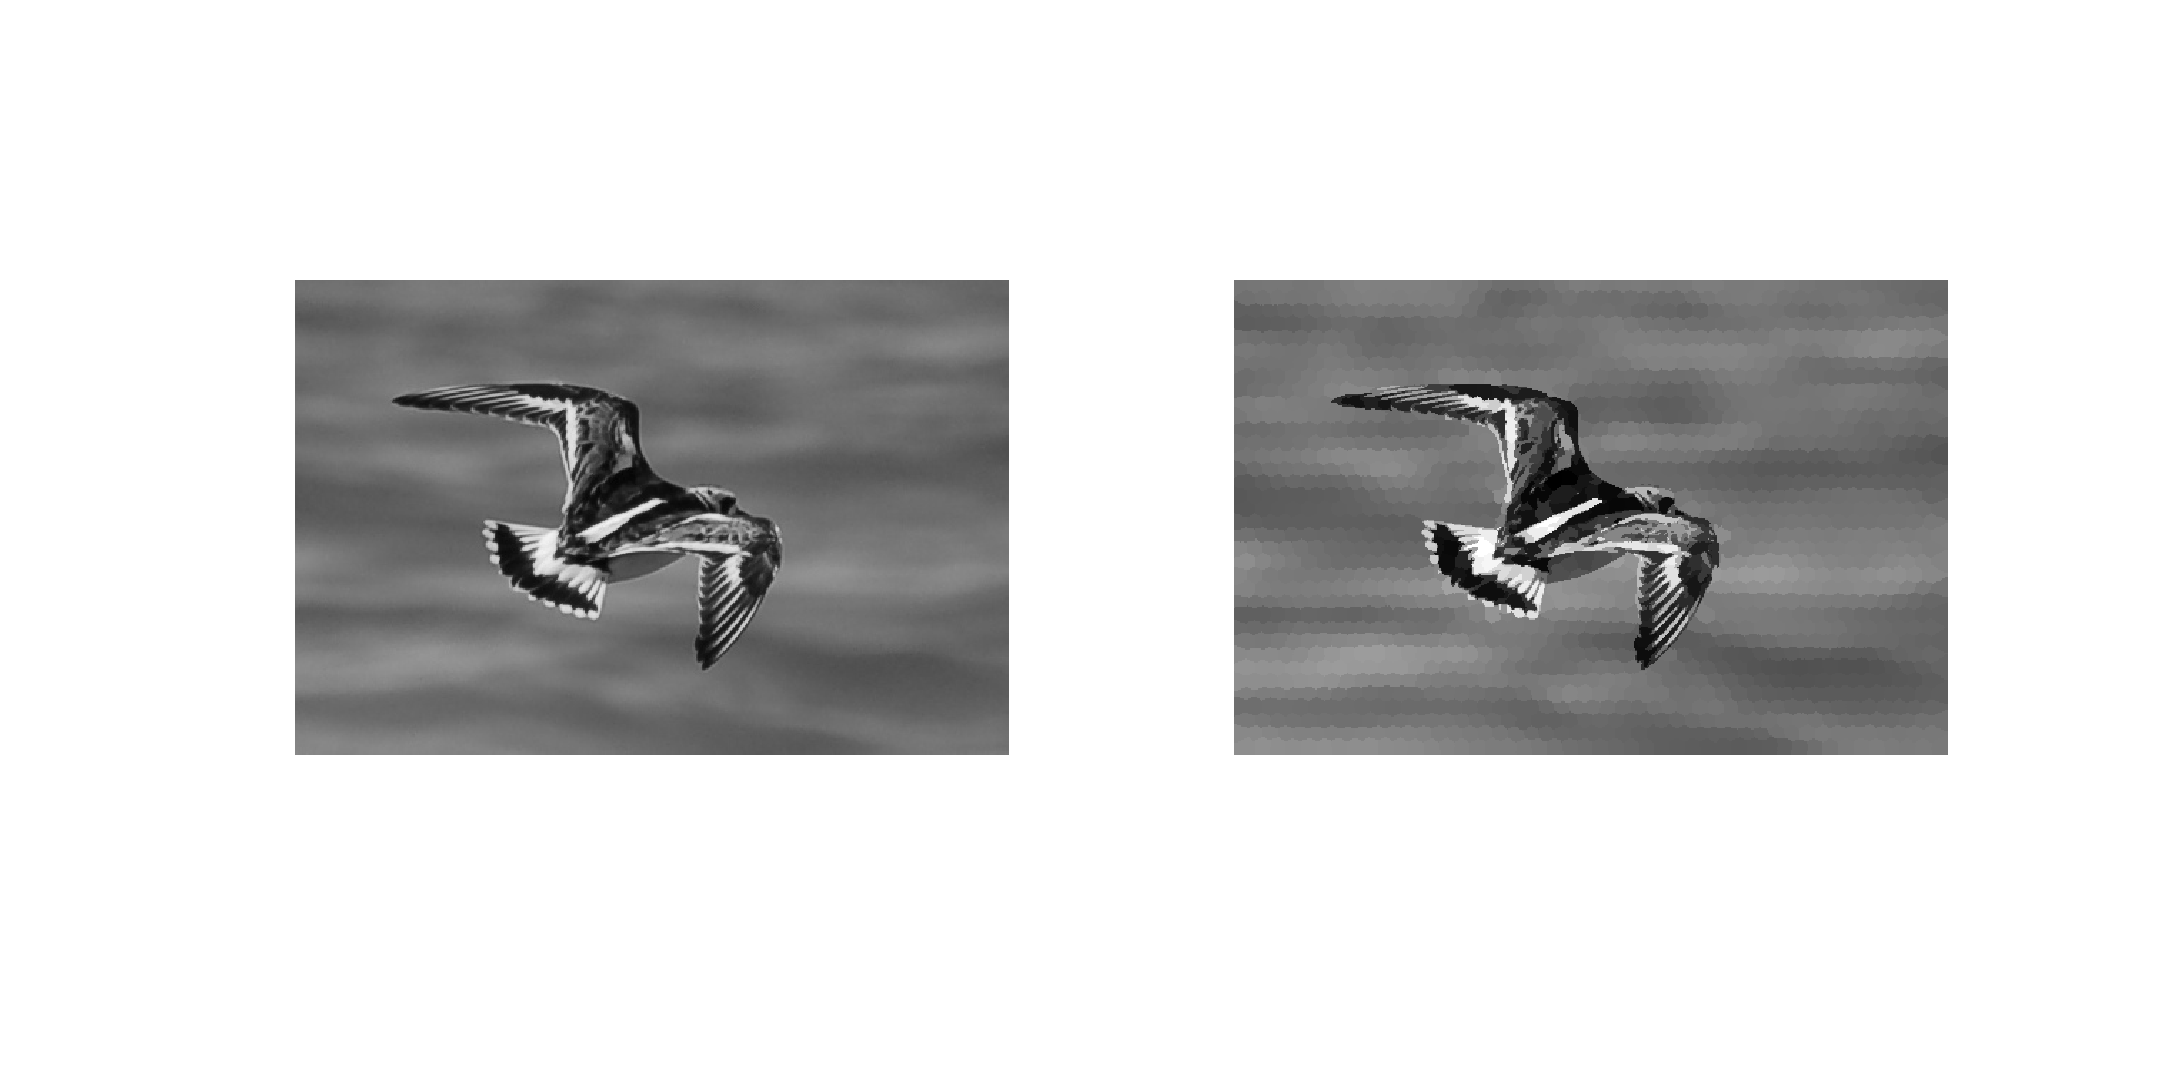
\includegraphics[width=0.85\textwidth]{superpixel_visualization.eps}
				\caption{Superpixel Visualization}
			\end{center}			
		\end{figure}

\end{frame}

\begin{frame}{Visualization}
		\begin{figure}[H]
			\begin{center}
				
\includegraphics[width=0.38\textwidth]{likelihood_rgb.eps}
				\caption{Visualization of Likelihood using RGB histogram}
			\end{center}			
		\end{figure}		
		\begin{figure}[H]
			\begin{center}
				
\includegraphics[width=0.38\textwidth]{likelihood_centroid.eps}
				\caption{Visualization of Likelihood based on distance from scribble}
			\end{center}			
		\end{figure}
\end{frame}
	

\begin{frame}{Visualization}	
	\begin{figure}[H]
		\begin{center}
			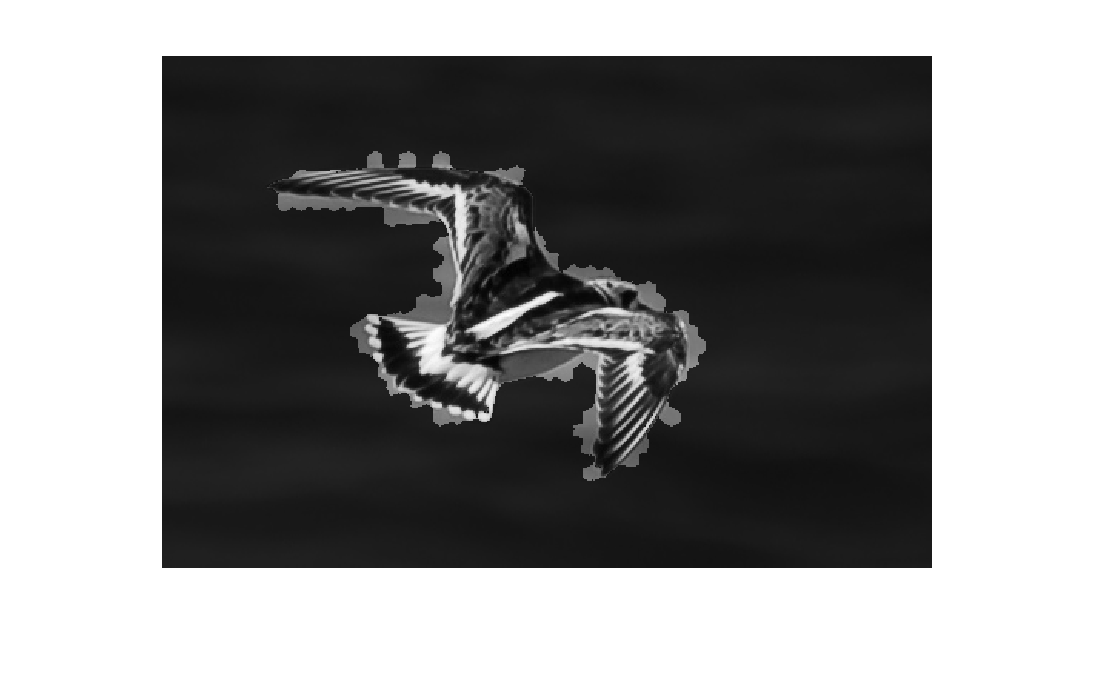
\includegraphics[width=0.60\textwidth]{likelihood_result.eps}
			\caption{Visualization of Max. Likelihood Estimation}
		\end{center}			
	\end{figure}
	
	\begin{itemize}
		\item {
			This result is obtained by max-likelihood estimation of how each superpixel is close to scribble in terms of rgb histogram and distance from scribble.
		}
	\end{itemize}
\end{frame}

	\subsection{Second Subsection}
	
	% You can reveal the parts of a slide one at a time
	% with the \pause command:	
	\begin{frame}{ Experiments}
		\begin{itemize}
			\item{
			\textbf{DATASET: Pascal VOC-2012} \\
			\begin{itemize}
				\item 20 classes segmentation
				\item scribble annotation available \newline
			\end{itemize}	
				
			}
		\item {
			"Dilation" Network built with Caffe. \newline
			Training: Pascal-VOC-2012 training data.
			\newline
		}			
		\item {
				Testing: 100 images from Pascal-VOC-2012 cross-validation set
			}
		\end{itemize}
	\end{frame}
	
	
	\begin{frame}{Experiment}
		\begin{itemize}
			\item{} \textbf{Evaluation Metric}
			
			\begin{align*}
			True \ positive \ rate \ = \frac{True \ positives(excl \  background)}{All \  positives(excl\ background)}
			\end{align*}
			
			\begin{block}{RESULTS}
			\begin{center}
				Mean Accuracy prior(Baseline) = 85.13 \\
				Mean Accuracy posterior(Ours) = 86.43					
			\end{center}
		\end{block}
		\end{itemize}
	\end{frame}	


	\begin{frame}{Visual Comparison}
			\begin{figure}[H]
				\begin{center}
					\includegraphics[width=1.00\textwidth]{man2.jpg}
					\caption{Baseline(left) vs Ours(right)}
				\end{center}			
			\end{figure}		
		\end{frame}
		

	\begin{frame}{Visual Comparison}
		\begin{figure}[H]
			\begin{center}
				\includegraphics[width=1.00\textwidth]{man1.jpg}
				\caption{Baseline(left) vs Ours(right)}
			\end{center}			
		\end{figure}		
	\end{frame}

	
	\begin{frame}{ Conclusion}
		\begin{itemize}
			\item {
				Incorporating information from scribbles increases segmentation accuracy even with a naive approach. \newline
			}
			\pause			
			\item{
				The improvement is significant for odd Neural Network outputs  \newline
			}
			\pause
			\item{
				 We can improve evaluation metric to focus on these odd outputs \newline
			}
			\pause
			\item{
				Also, we can improve label propagation methods from the scribbles.
			}
		\end{itemize}
	\end{frame}

	
	\begin{frame}{}
		\begin{itemize}
			\item[] \centering \textbf{Thank You!!}
		\end{itemize}
	\end{frame}
	
	
\end{document}